\begin{center}
	\begin{circuitfig}[H]
		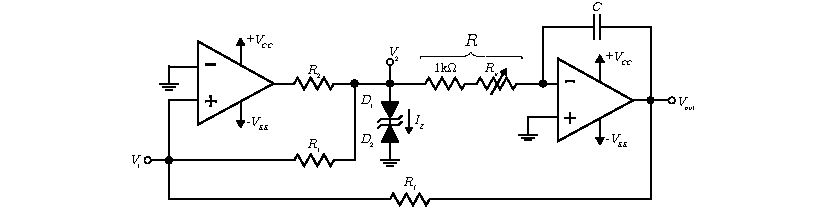
\includegraphics[width=14cm]{circuits/micro3_lab1.pdf}
		\caption{Γεννήτρια τριγωνικής παλμοσειράς.}
		\label{circ:1_schematic}
	\end{circuitfig}
\end{center}
\vspace*{-1cm}

Στην πρώτη άσκηση μελετάται το κύκλωμα \ref{circ:1_schematic} το οποίο αποτελείται από δύο τελεστικούς ενισχυτές μΑ741. Για την τροφοδοσία των τελεστικών ενισχυτών είναι $V_{CC}=15\unit{\volt}$ και $V_{EE}=15\unit{\volt}$. Οι δύο δίοδοι Zener (1N750) έχουν τάση Zener $V_Z=7.5\unit{\volt}$ και τάση στην ορθή πόλωση $V_D=0.7\unit{\volt}$.\par
Για τους ωμικούς αντιστάτες είναι $R_2=4.7\kohm$ και $R=40\kohm$. Για τις υπόλοιπες αντιστάσεις, $R_1,R_f$, και τον πυκνωτή $C$, βάσει των οδηγιών, προκύπτει $R_1=50\kohm$, $R_f=35\kohm$ και $C=4\unit{\nano\farad}$. Ωστόσο, επιλέχθηκαν οι πλησιέστερες τιμές που εμφανίζονται στα τυποποιημένα εξαρτήματα. Τελικά, το κύκλωμα υλοποιήθηκε με $R_1=47\kohm$, $R_f=33\kohm$ και $C=4.7\unit{\nano\farad}$.\par

\section{Θεωρητική μελέτη \& προσομοίωση}

	\subsection{Περιγραφή της λειτουργίας του κυκλώματος}
		Απαιτείται, από την εκφώνηση, το ύψος κάθε βήματος να είναι $0.6\unit{\volt}$, η διάρκεια του κάθε βήματος $t_s=4\unit{\ms}$, η ολική διάρκεια της κλίμακας να είναι $t_o=20\unit{\ms}$ και τέλος η χρονική απόσταση μεταξύ των κλιμάκων να είναι $t_{\mathrm{H}}=3\unit{\ms}$. Παρακάτω παρατίθεται, εν συντομία, ο υπολογισμός των $t_{\mathrm{on}}$, $t_{\mathrm{off}}$, $R_1$, $R_2$, $R_A$ και $R_B$. Η λεπτομερής θεωρητική ανάλυση του κυκλώματος και η επεξήγηση της λειτουργίας του γίνεται στην επόμενη ενότητα.\par
Ξεκινώντας από τον ολοκληρωτή φαίνεται εύκολα πως
\begin{equation*}
	0.6\unit{\volt}=\frac{2}{RC}\int_{t_a}^{t_b}{v_1(t)\dd{t}},
\end{equation*}
όπου $t_a$ είναι μία χρονική στιγμή κατά την οποία η έξοδος του 555, $v_1$, περνάει από LOW σε HIGH και $t_b=t_a+t_{\mathrm{on}}$, όπου $t_{\mathrm{on}}$ η διάρκεια ενός διαστήματος στο οποίο η $v_1$ παραμένει σε HIGH. Με αριθμητική αντικατάσταση προκύπτει
\begin{equation*}
	0.6\unit{\volt}=\frac{2}{10\kohm\cdot 1\unit{\micro\farad}}15\unit{\volt}\cdot t_{\mathrm{on}}\Rightarrow t_{\mathrm{on}}=400\unit{\micro\second}.
\end{equation*}

Εξαιτίας των διόδων στον ασταθή Α, ο πυκνωτής χωρητικότητας $C_1=0.1\unit{\micro\farad}$ φορτίζεται προς $V_{CC}$ μόνο μέσω της $R_1$ και εκφορτίζεται προς τη γείωση μόνο μέσω της $R_2$. Επομένως είναι $t_{\mathrm{on}}=0.693\cdot C_1\cdot R_1$ και $t_{\mathrm{off}}=0.693\cdot C_1\cdot R_2$. Επιπλέον, η συνολική διάρκεια ενός βήματος είναι $t_s=t_{\mathrm{on}}+t_{\mathrm{off}}$. Με αριθμητική αντικατάσταση στην τελευταία σχέση προκύπτει $t_{\mathrm{off}}=3.6\unit{\ms}$.
\begin{equation*}
	R_1=\frac{t_{\mathrm{on}}}{0.693\cdot C_1}=\frac{0.4\unit{\ms}}{0.693\cdot 0.1\unit{\micro\farad}}\Rightarrow R_1=5.772\kohm
\end{equation*}
και
\begin{equation*}
	R_2=\frac{t_{\mathrm{off}}}{0.693\cdot C_1}=\frac{3.6\unit{\ms}}{0.693\cdot 0.1\unit{\micro\farad}}\Rightarrow R_2=51.948\kohm.
\end{equation*}

Περνώντας στον ασταθή πολυδονητή Β, ο πυκνωτής χωρητικότητας $C_2=0.1\unit{\micro\farad}$ φορτίζεται μέσω της $R_A$ και εκφορτίζεται προς τη γείωση μέσω της $R_B$. Συνεπώς, $t_o=t_{\mathrm{L}}=1.1R_B\cdot C_2$ και $t_{\mathrm{H}}=1.1R_A\cdot C_2$. Δηλαδή
\begin{equation*}
	R_Α=\frac{t_{\mathrm{H}}}{1.1\cdot C_2}=\frac{3\unit{\ms}}{1.1\cdot 0.1\unit{\micro\farad}}\Rightarrow R_A=27.272\kohm
\end{equation*}
και
\begin{equation*}
	R_B=\frac{t_{\mathrm{L}}}{1.1\cdot C_2}=\frac{20\unit{\ms}}{1.1\cdot 0.1\unit{\micro\farad}}\Rightarrow R_B=181.818\kohm.
\end{equation*}

	\subsection{Θεωρητικός σχεδιασμός κυματομορφών}
		\subsubsection{Ασταθής πολυδονητής Α}
	Το τερματικό 2 του 555 είναι το trigger $\mathrm{(TR)}$ και το τερματικό 6 είναι το threshold $\mathrm{(TH)}$. Όταν το 555 λαμβάνει ενεργό σήμα $\overline{\mathrm{TR}}$ η έξοδος του περνάει στο HIGH, κοντά στην τάση τροφοδοσίας $V_{CC}$ και παραμένει εκεί για χρόνο $t_{\mathrm{on}}$ έως ότου να παρουσιαστεί ενεργό σήμα $\mathrm{TH}$. Τότε, η έξοδος του 555 περνάει στο LOW, κοντά στη γείωση.\cite{artofelectronics}\par
	Το $\overline{\mathrm{TR}}$ ενεργοποιείται από τάση μικρότερη του $\frac{1}{3}V_{CC}$, ενώ το $\mathrm{TH}$ από τάση μεγαλύτερη των $\frac{2}{3}V_{CC}$.\cite{artofelectronics}\cite{sedra}\cite{scherz}\par
	Ο πυκνωτής $C_1$ αρχίζει να φορτίζεται προς $V_{CC}$ μόλις το κύκλωμα συνδεθεί στην τροφοδοσία.\cite{scherz} Η φόρτισή του, λόγω των δύο διόδων, γίνεται μόνο μέσω του ωμικού αντιστάτη $R_1$. Η έξοδος του χρονιστή 555 βρίσκεται σε στάθμη HIGH όσο ο πυκνωτής φορτίζεται. Μόλις ο πυκνωτής $C_1$ ξεπεράσει τα $\frac{2}{3}V_{CC}$ το σήμα $\mathrm{TH}$ γίνεται ενεργό και το $\overline{\mathrm{TR}}$ απενεργοποιείται, οδηγώντας την έξοδο σε στάθμη LOW για χρονικό διάστημα $t_{\mathrm{off}}$, και ο πυκνωτής αρχίζει να εκφορτίζεται, μέσω του $R_2$, προς τη γείωση.\cite{artofelectronics}\par
	Βάσει των παραπάνω, η τάση του πυκνωτή $C_1$ είναι $\frac{1}{3}V_{CC}\leqslant v_{C_1}\leqslant\frac{2}{3}V_{CC}$ και η περίοδος του παλμού\footnote{Εάν δεν υπήρχαν οι δίοδοι θα ήταν $T=0.693\cdot\(R_1+2R_2\)$.\cite{artofelectronics}\cite{sedra}\cite{scherz}} είναι $T=t_s=0.693\cdot(R_1+R_2)\cdot C_1$. Εφόσον είναι $T=t_s=t_{\mathrm{on}}+t_{\mathrm{off}}$ και οι δίοδοι ορίζουν δύο ξεχωριστές διαδρομές για τη φόρτιση και την εκφόρτιση του πυκνωτή, θα είναι $t_{\mathrm{on}}=0.693\cdot R_1\cdot C_1$ και $t_{\mathrm{off}}=0.693\cdot R_2\cdot C_1$. Τέλος, ο κύκλος εργασίας (duty cycle), $\sfrac{t_{\mathrm{on}}}{t_s}$, είναι προφανές πως ισούται με $\sfrac{R_1}{\(R_1+R_2\)}$.\par
	% TODO:
	% + διάγραμμα V1
\subsubsection{BJT $T_2$}
	Το BJT $T_2$ εξασφαλίζει τον συγχρονισμό μεταξύ των δύο ταλαντωτών Α και Β. Ο χρονιστής 555 λειτουργεί όσο το reset (R) (ακροδέκτης 4) είναι συνδεδεμένο στην τροφοδοσία, $V_{CC}$. Προκειμένου να σταματήσουμε την παραγωγή των παλμών του ασταθούς Α και να ξεκινήσει εκ νέου η παραγωγή της κλίμακας, $v_{\mathrm{out}}$, πρέπει το reset να πάρει τιμή κοντά στη γείωση. Δηλαδή πρέπει να είναι ενεργό το $\overline{\mathrm{R}}$.\par
	Όταν η έξοδος του ασταθούς Β βρίσκεται στην υψηλή στάθμη, κατά συνέπεια και η $v_3$, σταματά η παραγωγή της κλίμακας $u_{\mathrm{out}}$. Επομένως, μέσω αντίστασης, η $v_3$ συνδέεται στην βάση του $T_2$ το οποίο ξεκινά να άγει στην περιοχή του κορεσμού και εφαρμόζει στον ακροδέκτη reset του 555 μία τάση κοντά στη γείωση, $v_{CE}$.

\subsubsection{Ασταθής πολυδονητής Β}
	Ο ασύμμετρος ασταθής πολυδονητής Β υλοποιείται χρήσει τελεστικού ενισχυτή μA741. Έστω $L_+$ η υψηλή στάθμη της εξόδου του πολυδονητή και $L_-$ η χαμηλή στάθμη του πολυδονητή. Οι δύο αυτές καταστάσεις της εξόδου χαρακτηρίζονται ως ημισταθείς \textsl{(quasi-stable states)}\cite{sedra}και η διάρκειά τους εξαρτάται από τις χρονικές σταθερές του δικτύου $R_AR_BC_2$ και από τις τάσεις κατωφλίου του πολυδονητή.\cite{sedra}\par
	Έστω πως η λειτουργία του κυκλώματος ξεκινά με την έξοδο του πολυδονητή στην υψηλή στάθμη $L_+$, είναι δηλαδή $v_2=L_+$. Τότε, μέσω της $R_A$ ο πυκνωτής $C_2$ αρχίζει να φορτίζεται προς $L_+$. Επομένως, η τάση στην αναστρέφουσα είσοδο του τελεστικού ενισχυτή αυξάνεται εκθετικά προς $L_+$ ως εξής
	\begin{equation}
		\label{eq:ask2:B:inverting:high}
		v_-=L_+-\(L_+-\beta L_-\)\exp{\(-\sfrac{t}{\tau_+}\)},
	\end{equation}
	όπου $\beta=\frac{R_i}{R_f+R_i}$\cite{sedra}\cite{jaeger} που προκύπτει από τον διαιρέτη τάσης μεταξύ της εξόδου και της μη αναστρέφουσας εισόδου του τελεστικού ενισχυτή και $\tau_+=R_A\cdot C_2$ η χρονική σταθερά φόρτισης του πυκνωτή. Ταυτόχρονα, η τάση στην μη αναστρέφουσα είσοδο του τελεστικού ενισχυτή είναι $v_+=\beta\cdot L_+$.\par
	Μόλις η τάση στα άκρα του πυκνωτή φτάσει την άνω τάση κατωφλίου $V_{UTP}=\beta\cdot L_+$\cite{sedra} ο πολυδονητής αλλάζει κατάσταση και η έξοδός του περνά στη χαμηλή στάθμη $v_2=L_-$. Η τάση στη μη αναστρέφουσα είσοδο του τελεστικού είναι $v_+=\beta\cdot L_+$ και ο πυκνωτής $C_2$ εκφορτίζεται, μέσω της $R_B$ προς $L_-$. Επομένως, η τάση στην αναστρέφουσα είσοδο του τελεστικού ενισχυτή μειώνεται εκθετικά προς $L_-$ ως εξής
	\begin{equation}
		\label{eq:ask2:B:inverting:low}
		v_-=L_--\(L_--\beta L_+\)\exp{\(-\sfrac{t}{\tau_-}\)},
	\end{equation}
	όπου $\tau_-=R_B\cdot C_2$ η χρονική σταθερά εκφόρτισης του πυκνωτή. Μόλις η τάση στην αναστρέφουσα είσοδο φτάσει την κάτω τάση κατωφλίου $V_{LTP}=\beta\cdot L_-$\cite{sedra} ο πολυδονητής αλλάζει και πάλι κατάσταση και η έξοδός του, $v_2$, περνάει στην υψηλή στάθμη $L_+$.\par
	Από τη σχέση \eqref{eq:ask2:B:inverting:high} αντικαθιστώντας $v_-=\beta\cdot L_+=V_{UTP}$ προκύπτει πως η έξοδος του πολυδονητή παραμένει στην θετική στάθμη για χρόνο
	\begin{equation}
		t_{\mathrm{H}}=R_A\cdot C_2\cdot\ln{\left[\frac{1-\beta\(\sfrac{L_-}{L_+}\)}{1-\beta}\right]}.
	\end{equation}

	Ομοίως, από τη σχέση \eqref{eq:ask2:B:inverting:low} προκύπτει πως η έξοδος του πολυδονητή παραμένει στην αρνητική στάθμη για χρόνο
	\begin{equation}
		t_{\mathrm{L}}=R_B\cdot C_2\cdot\ln{\left[\frac{1-\beta\(\sfrac{L_+}{L_-}\)}{1-\beta}\right]}.
	\end{equation}

	Στην περίπτωση που $L+\cong -L_-$ τότε η περίοδος $T$ του πολυδονητή είναι
	\begin{equation*}
		T=t_{\mathrm{H}}+t_{\mathrm{L}}=\(R_A+R_B\)\cdot C_2\cdot\ln{\(\frac{1+\beta}{1-\beta}\)}.
	\end{equation*}

	Η δημιουργία δύο διαφορετικών μονοπατιών φόρτισης και εκφόρτισης του πυκνωτή $C_2$, χρήσει των διόδων, επιτρέπει την προσαρμογή του duty cycle σε οποιοδήποτε επιθυμητό ποσοστό.\par

\subsubsection{Ολοκληρωτής}
	Για τα ρεύματα στο σχήμα του ολοκληρωτή ισχύει $i_i=i_f+i_C\Longleftrightarrow i_C=i_i-i_f$ (Kirchhoff's current law). Από τον νόμο του Ohm εύκολα προκύπτει πως
	\begin{equation*}
		i_i=\frac{v_1-v_c}{R}\quad\land\quad i_f=\frac{v_c-v_{\mathrm{out}}}{R},\quad R=10\kohm.
	\end{equation*}
	Συνεπώς,
	\begin{equation*}
		i_C=\frac{v_1-v_c-\(v_c-v_{\mathrm{out}}\)}{R}=\frac{v_1+v_{\mathrm{out}}-2v_c}{R}.
	\end{equation*}

	Με αντικατάσταση της παραπάνω έκφρασης του ρεύματος $i_C$ στη σχέση τάσης---ρεύματος πυκνωτή $v_c=\displaystyle{\frac{1}{C}\int{i_C\dd{t}}}$ έχουμε
	\begin{equation*}
		v_c=\frac{1}{C}\int{\frac{v_1+v_{\mathrm{out}}-2v_c}{R}\dd{t}}
	\end{equation*}
	ή
	\begin{equation}\label{eq:ask2:vc:int}
		v_c=\frac{1}{R\cdot C}\int{\(v_1+v_{\mathrm{out}}-2v_c\)\dd{t}}
	\end{equation}
	Aπό τον διαιρέτη τάση στο δίκτυο ανάδρασης της αναστρέφουσας εισόδου του τελεστικού ενισχυτή προκύπτει πως $v_-=\frac{R}{R+R}v_{\mathrm{out}}\Longleftrightarrow v_-=\frac{1}{2}v_{\mathrm{out}}$. Ο τελεστικός ενισχυτής θεωρούμε πως βρίσκεται στη γραμμική περιοχή λειτουργίας του. Επομένως, η τάση της μη αναστρέφουσας εισόδου του είναι ίση με την τάσης της αναστρέφουσας εισόδου, δηλαδή $v_+=v_-=v_c$. Τότε θα είναι
	\begin{equation}\label{eq:ask2:vout:vc}
		v_c=\frac{1}{2}v_{\mathrm{out}}.
	\end{equation}
	Αντικαθιστώντας τη σχέση \eqref{eq:ask2:vout:vc} στη σχέση \eqref{eq:ask2:vc:int} έχουμε
	\begin{equation}
		\label{eq:ask2:integrator:vout:v1}
		v_{\mathrm{out}}(t)=\frac{2}{R\cdot C}\int{v_1(t)\dd{t}}.
	\end{equation}
	Η σχέση \eqref{eq:ask2:integrator:vout:v1} είναι που δικαιολογεί τη λειτουργία του κυκλώματος ως ολοκληρωτή.\par

\subsubsection{BJT $T_1$}
	 Όσο η έξοδος του του ασταθούς Β είναι στη χαμηλή στάθμη, το $T_1$ είναι σε αποκοπή. Όταν η έξοδος του ασταθούς Β περνά στην υψηλή στάθμη, το $T_1$ ξεκινά να άγει και εισέρχεται στον κορεσμό και ο πυκνωτής $C$ αρχίζει την εκφόρτιση προς τη γείωση.\par

\subsubsection{Συνολική λειτουργία}
	Στην έξοδο του κυκλώματος, $v_{\mathrm{out}}$, περιοδικά εμφανίζεται κλίμακα τάσης.\par
	Η έξοδος του ασταθούς πολυδονητή Α συνδέεται μέσω αντίστασης R στη μη αναστρέφουσα είσοδο του τελεστικού ενισχυτή του ολοκληρωτή και στον πυκνωτή $C$ του ολοκληρωτή. Όσο η έξοδος του πολυδονητή Α, $v_1$, είναι στην υψηλή στάθμη ο πυκνωτής $C$, του κυκλώματος του ολοκληρωτή, φορτίζεται και εκτελείται η πράξη της ολοκλήρωσης. Όσο η έξοδος του πολυδονητή Α είναι στο μηδέν το κύκλωμα του ολοκληρωτή διατηρεί σταθερή την τάση στην έξοδό του. Επομένως, η συνολική διάρκεια ενός βήματος είναι $t_s=t_{\mathrm{on}}+t_{\mathrm{off}}$ η οποία ισούται με την περίοδο του ασταθούς Α.\par
	Η παραγωγή της κλίμακας πραγματοποιείται όταν η τάση $v_3$ είναι μηδέν. Εξαιτίας της διόδου στην έξοδο του ασταθούς πολυδονητή Β, η $v_3=0$ ισοδυναμεί με $v_2$ στη χαμηλή στάθμη. Επομένως, η διάρκεια της κλίμακας είναι \begin{equation*}
		t_{\mathrm{L}}=R_B\cdot C_2\cdot\ln{\left[\frac{1-\beta\(\sfrac{L_+}{L_-}\)}{1-\beta}\right]}
	\end{equation*}
	και η απόσταση μεταξύ των κλιμάκων είναι \begin{equation*}
		t_{\mathrm{H}}=R_A\cdot C_2\cdot\ln{\left[\frac{1-\beta\(\sfrac{L_-}{L_+}\)}{1-\beta}\right]}.
	\end{equation*}

	Το ύψος κάθε βήματος καθορίζεται από τον ολοκληρωτή ως εξής
	\begin{equation*}
		V_{\mathrm{step}}=\frac{2}{R\cdot C}\int_{t_a}^{t_b}{v_1(t)\dd{t}},
	\end{equation*}
	όπου $t_a$ είναι μια χρονική στιγμή στην οποία η $v_1$ περνάει από μηδέν σε υψηλή σταθμη και $t_b=t_a+t_{\mathrm{on}}$.\par

	% Q4
	\subsection{Προσομοίωση με PSpice}
		\vspace*{-0.35cm}
\begin{center}
	\begin{circuitfig}[H]
		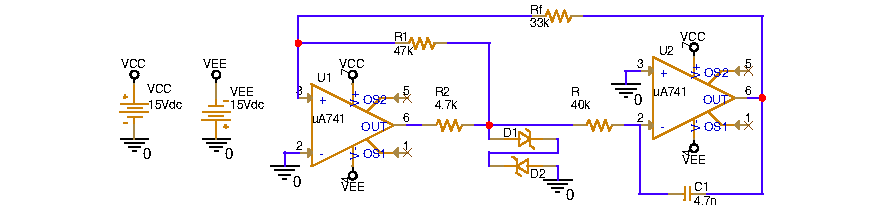
\includegraphics[width=14cm]{spice_01/schematic.pdf}
		\caption{Κύκλωμα προσομοίωσης για το PSpice.}
		\label{circ:spice:1_schematic}
	\end{circuitfig}
\end{center}
\vspace*{-20pt}

Οι προσομοιώσεις έγιναν με το κύκλωμα \ref{circ:spice:1_schematic}. Οι δίοδοι Zener\footnote{Χρησιμοποιήθηκαν δεδομένα από data sheet της διόδου 1N5236B του εμπορίου.}, D1 και D2, δημιουργήθηκαν χρήσει του \textsl{PSpice Modeling Application}. Η τάση Zener των διόδων ορίστηκε $V_Z=7.5\unit{\volt}$ και ο θερμοκρασιακός συντελεστής ορίσθηκε στο $0.058\displaystyle{\sfrac{\%}{\unit{\celsius}}}$.

Οι περίοδοι των κυματομορφών βρέθηκαν με τη βοήθεια των cursors ενώ τα μέγιστα και ελάχιστα των κυματομορφών βρέθηκαν χρήσει των συναρτήσεων \texttt{Max()} και \texttt{Min()}. Τα αποτελεσματα φαίνονται στον πίνακα \ref{table:ask1:q4:periods}.

\begin{table}[h]
	\begin{center}
		\begin{tabular}{|c|c|c|c|c|}
			\specialrule{1.25pt}{0pt}{0pt}
			\textbf{Σήμα}      & \textbf{Περίοδος}             & \textbf{Μέγιστη τιμή}         & \textbf{Ελάχιστη τιμή}         & \textbf{Πλάτος}                             \\
			\hline
			\hline
			$v_1$              & $670.669\unit{\micro\second}$ & $7.02052\unit{\volt}$         & $-7.01512\unit{\volt}$         & $14.03564\unit{\volt}_{\mathrm{pp}}$        \\\hline
			$v_2$              & $670.707\unit{\micro\second}$ & $8.06550\unit{\volt}$         & $-8.06549\unit{\volt}$         & $16.13099\unit{\volt}_{\mathrm{pp}}$        \\\hline
			$v_{\mathrm{out}}$ & $670.707\unit{\micro\second}$ & $6.77889\unit{\volt}$         & $-6.77670\unit{\volt}$         & $13.55559\unit{\volt}_{\mathrm{pp}}$        \\\hline
			$i_z$              & $670.709\unit{\micro\second}$ & $1.20446\unit{\milli\ampere}$ & $-1.20582\unit{\milli\ampere}$ & $2.41028\unit{\milli\ampere}_{\mathrm{pp}}$ \\\specialrule{1.25pt}{0pt}{0pt}
		\end{tabular}
		\caption{Μετρήσεις των κυματομορφών του διαγράμματος \ref{plot:ask1:q4}.}
		\label{table:ask1:q4:periods}
	\end{center}
\end{table}

\begin{plot_fig}[H]
	\begin{center}
		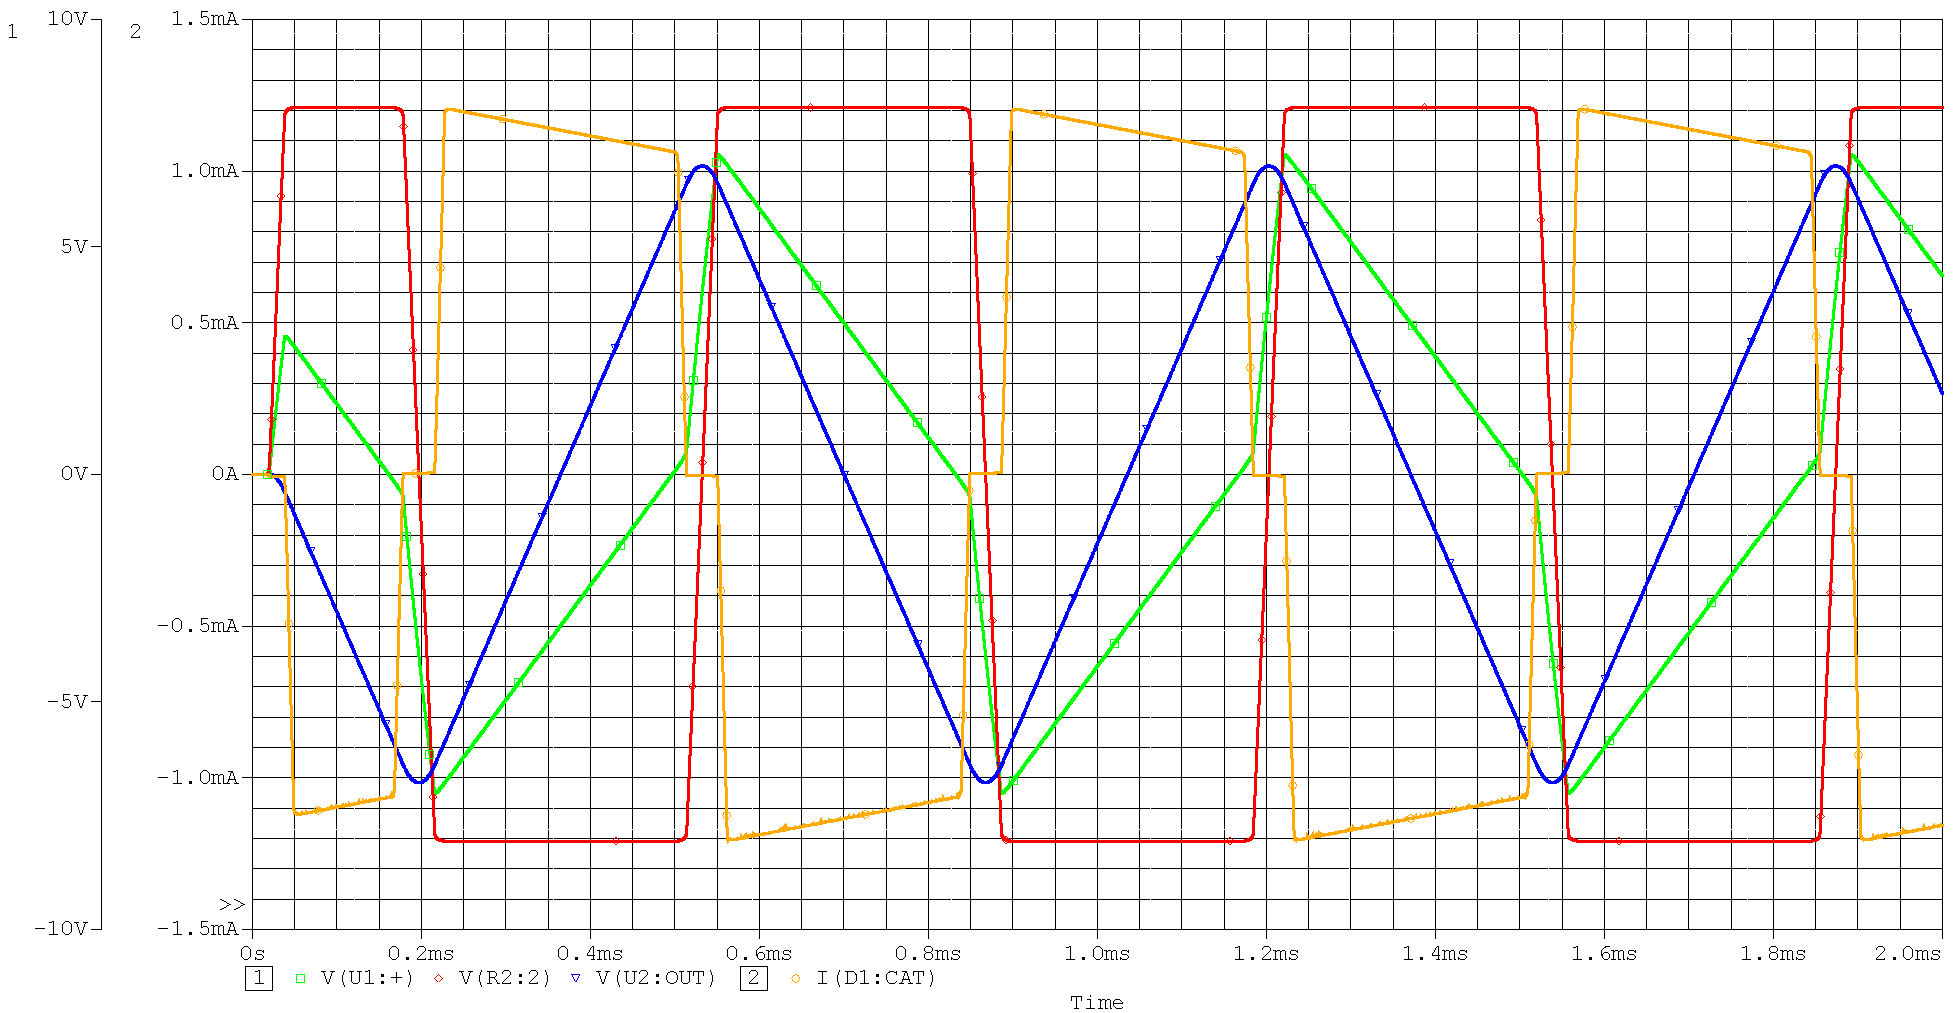
\includegraphics[width=15cm]{spice_01/q4.pdf}
		\caption{Οι τάσεις $v_1$ (πράσινη κυματομορφή), $v_2$ (κόκκινη κυματομορφή) και $v_{\mathrm{out}}$ (μπλε κυμματομορή) και το ρεύμα $i_z$ (πορτοκαλί κυματομορφή).}
		\label{plot:ask1:q4}
	\end{center}
\end{plot_fig}


	\subsection{Μέγιστη συχνότητα λειτουργίας I}
		Έγινε προσομοίωση του κυκλώματος στις θερμοκρασίες $-20\unit{\celsius}$, $0\unit{\celsius}$, $20\unit{\celsius}$, $35\unit{\celsius}$ και $70\unit{\celsius}$ και παρατηρήθηκε η κυματομορφή της εξόδου. Τα αποτελέσματα φαίνονται στο διάγραμμα \ref{plot:2_temp}.\par

\begin{table}[h]
	\begin{center}
		\begin{tabular}{|l |c |c |c |c |c |}
			\specialrule{1.25pt}{0pt}{0pt}
			\textbf{PSpice measurement} & $-20\unit{\celsius}$           & $0\unit{\celsius}$             & $20\unit{\celsius}$            & $35\unit{\celsius}$            & $70\unit{\celsius}$            \\\hline\hline
			\texttt{Max(V(U2:OUT))}     & $6.79172\unit{\volt}$          & $6.76318\unit{\volt}$          & $6.72997\unit{\volt}$          & $6.68878\unit{\volt}$          & $6.63272\unit{\volt}$          \\\hline
			\texttt{Period(V(U2:OUT))}  & $23.84931\unit{\milli\second}$ & $23.75302\unit{\milli\second}$ & $23.65926\unit{\milli\second}$ & $23.58503\unit{\milli\second}$ & $23.37579\unit{\milli\second}$ \\\specialrule{1.25pt}{0pt}{0pt}
		\end{tabular}
		\caption{Μετρήσεις των κυματομορφών του διαγράμματος \ref{plot:2_temp}.}
		\label{table:ask2:q5}
	\end{center}
\end{table}

Από τον πίνακα \ref{table:ask2:q5} προκύπτει πως η αύξηση της θερμοκρασίας μειώνει την μέγιστη τάση της κλίμακας αλλά μειώνει και την περίοδό της. Από το διάγραμμα \ref{plot:2_temp} φαίνεται πως η αύξηση της θερμοκρασίας μετατοπίζει την κυματομορφή ελαφρώς προς τα αριστερά.\par

\begin{plot_fig}
	\centering
	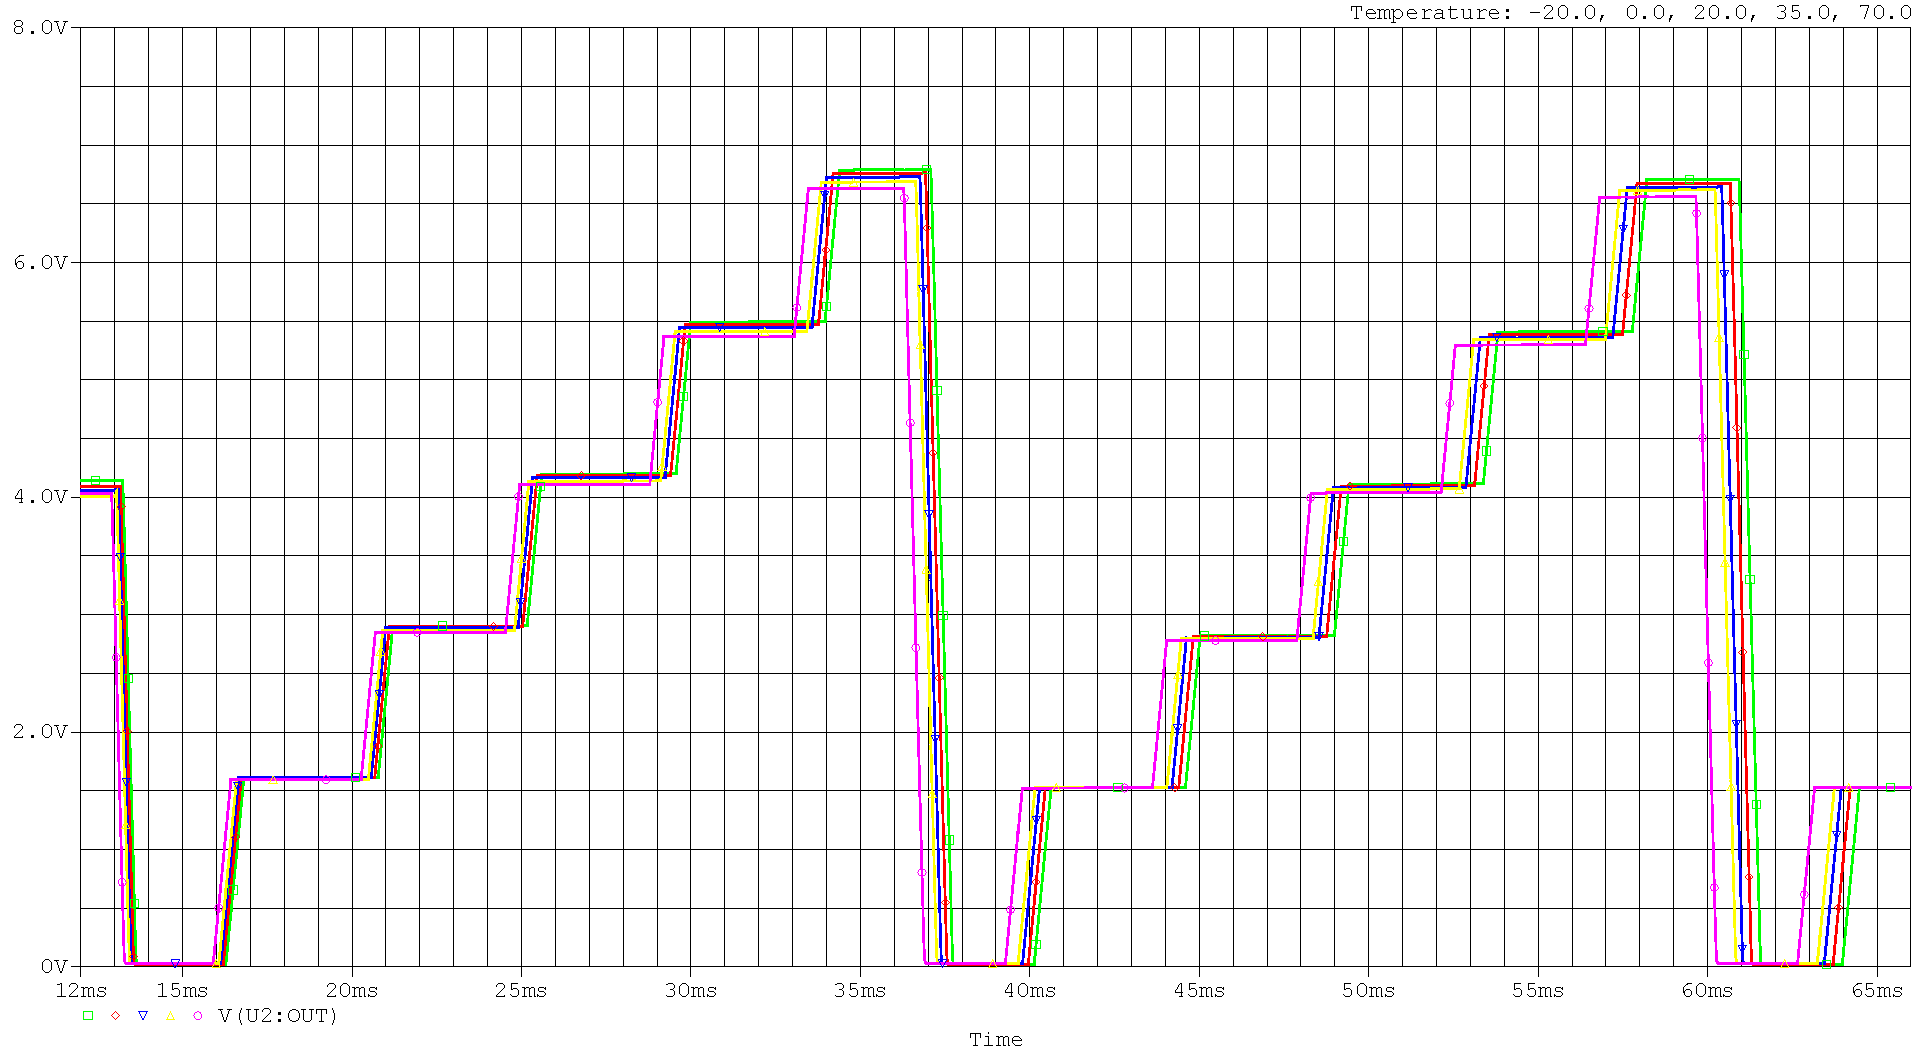
\includegraphics[width=13cm]{spice_02/q5.pdf}
	\caption{Temperature sweep. Οι κυματομορφές στο υπόμνημα, από αριστερά προς δεξιά, αντιστοιχούν στις θερμοκρασίες $-20\unit{\celsius}$, $0\unit{\celsius}$, $20\unit{\celsius}$, $35\unit{\celsius}$ και $70\unit{\celsius}$.}
	\label{plot:2_temp}
\end{plot_fig}
\vspace*{1cm}

	\subsection{Μέγιστη συχνότητα λειτουργίας II}
		\setlength{\columnsep}{2pt}
\setlength{\columnseprule}{0pt}
\begin{multicols}{2}
	Η μεταβολή του ρεύματος στη βάση του transistor επιτυγχάνεται μέσω της μεταβολής της τάσης στην έξοδο της γεννήτριας. Η εναλλασσόμενη πηγή τάσης \texttt{Vce} έχει περίοδο $T_{v_{CE}}=\sfrac{1}{1\unit{\kilo\hertz}}=1\unit{\milli\second}$ αρκετά μικρότερη από την διάρκεια κάθε βήματος της γεννήτριας, $t_s\simeq4.5\unit{\milli\second}$. Επομένως, το ρεύμα στη βάση του transistor παραμένει σταθερό για αρκετό χρόνο ώστε να ολοκληρωθεί η σάρωση της διαφοράς δυναμικού μεταξύ συλλέκτη και εκπομπού.\par
	Η προσομοίωση γίνεται στο πεδίο του χρόνου σε διάστημα μίας περιόδου της κλιμακωτής τάσης. Μέσω των ρυθμίσεων των αξόνων στο PSpice, επιλέγεται η διαφορά δυναμικού μεταξύ συλλέκτη και εκπομπού ως η μεταβλητή του οριζόντιου άξονα. Ως \texttt{trace} του γραφήματος επιλέγεται το ρεύμα στον εκπομπό. Τα αποτελέσματα της προσομοίωσης φαίνονται στο διάγραμμα \ref{plot:2_bjt}.\par
	\begin{center}
		\begin{circuitfig}[H]
			\centering
			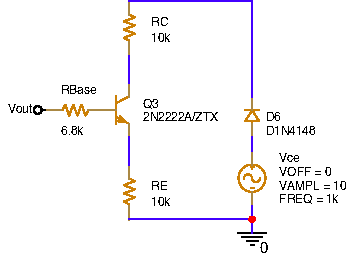
\includegraphics[width=5cm]{spice_02/ask2_bjt_schematic.pdf}
			\caption{Κύκλωμα για τη λήψη των χαρακτηριστικών $v_{CE}-i_C$ ενός BJT. Το κύκλωμα συνδέεται στην έξοδο της γεννήτριας κλιμακωτής τάσης.}
			\label{circ:2_bjt_schematic}
		\end{circuitfig}
	\end{center}
\end{multicols}
\vspace*{-0.35cm}
\begin{plot_fig}[H]
	\begin{center}
		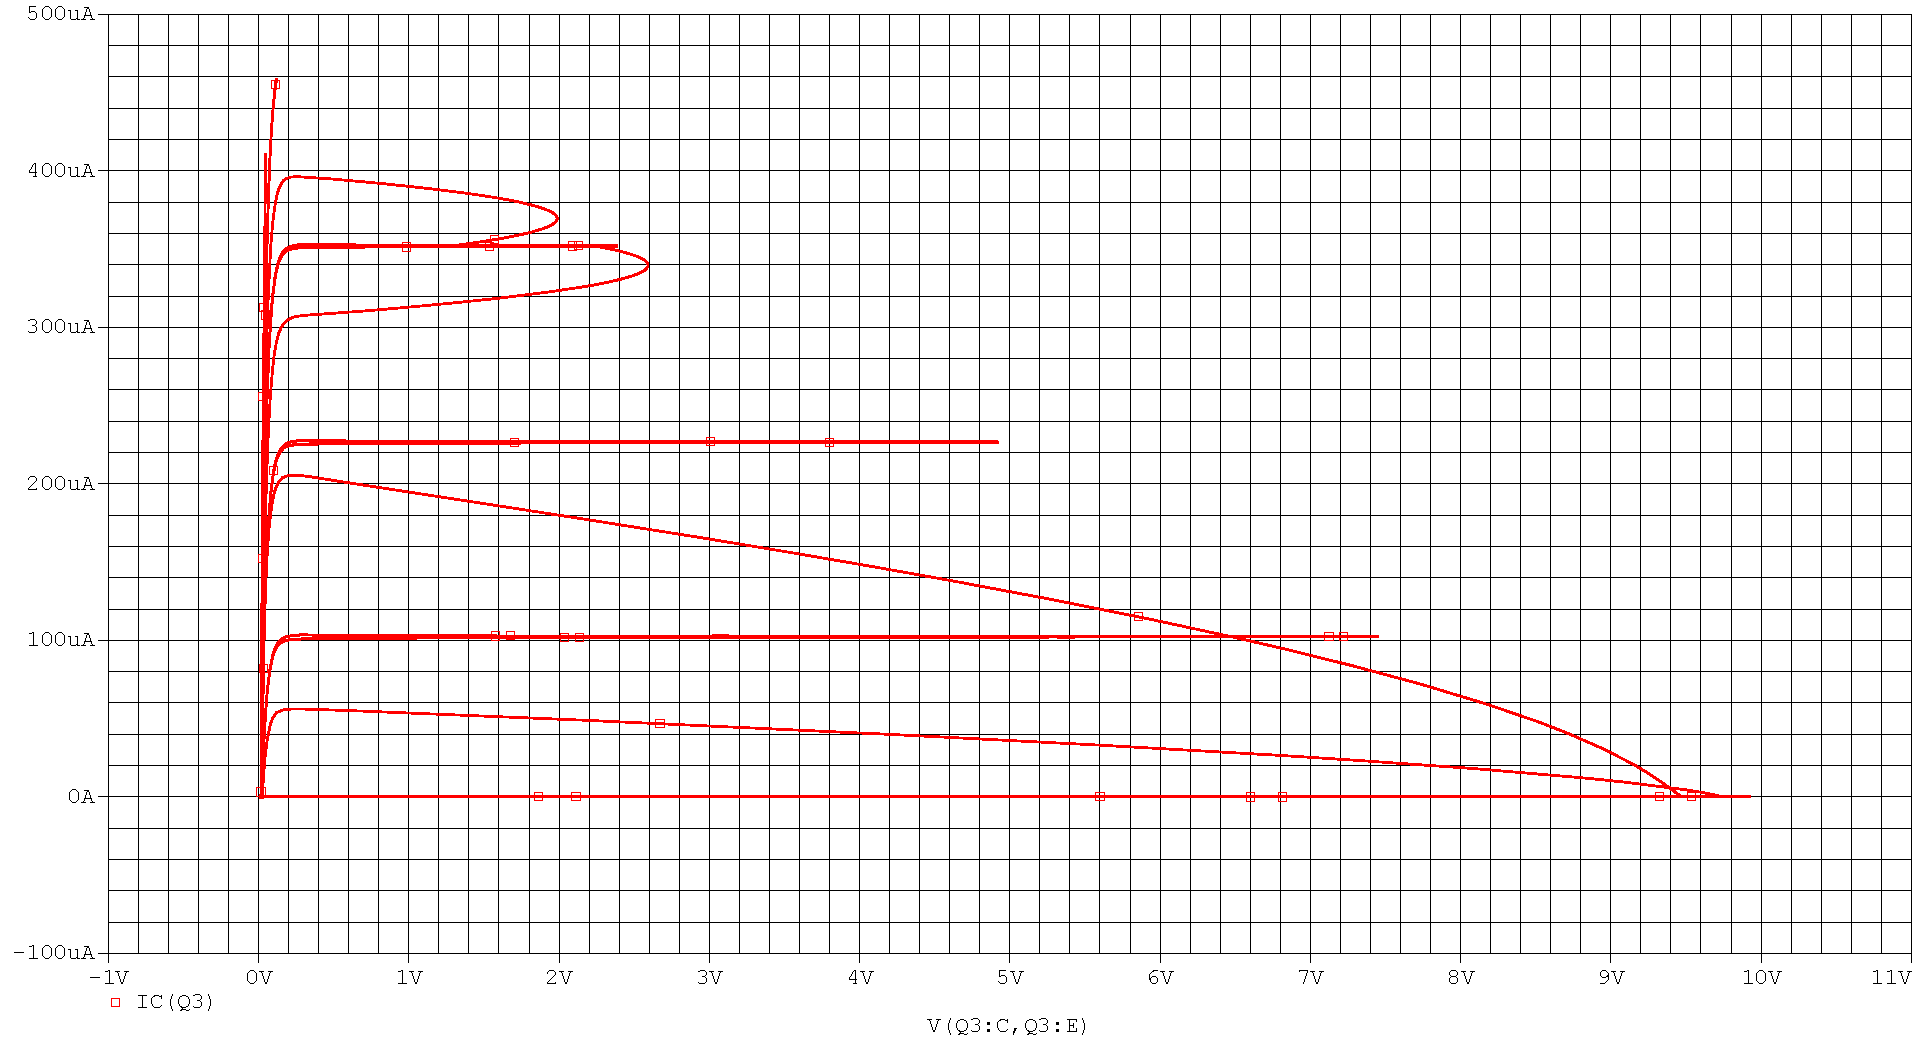
\includegraphics[height=5.5cm]{spice_02/q6.pdf}
		\caption{Χαρακτηριστικές $v_{CE}-i_C$. Οι \textsl{ενδιάμεσες} καμπύλες, μεταξύ των αναμενόμενων καμπυλών, οφείλονται στο γεγονός πως καθώς μεταβάλλεται η έξοδος της γεννήτριας η σάρωση της πηγής \texttt{Vce} του κυκλώματος \ref{circ:2_bjt_schematic} συνεχίζεται.}
		\label{plot:2_bjt}
	\end{center}
\end{plot_fig}

	\subsection{Ρύθμιση πλάτους εξόδου}
		Σύμφωνα με την σχέση \eqref{eq:ask1_vout} το πλάτος του τριγωνικού παλμού μπορεί να ρυθμιστεί μεταβάλλοντας την κλίση του. Αυτό είναι δυνατό αν τροποποιήσουμε τις μεταβλητές $R_f$ και $R_1$. Λαμβάνοντας ωστόσο υπόψιν την σχέση \eqref{eq:ask1_freq} οι μεταβλητές αυτές θα μεταβάλλουν την συχνότητα. Για να ρυθμιστεί το πλάτος χωρίς να αλλάξει η συχνότητα, πρέπει να αλλάξει το όριο της $v_2$, το οποίο εξαρτάται από τις διόδους Zener και ισούται με $-\(V_D+V_Z\)$. Οπότε χρησιμοποιώντας διόδους με διαφορετικές τάσεις Zener και threshold θα μπορέσουν να ρυθμίσουν το πλάτος του παλμού, δίχως να μεταβληθεί η συχνότητα.

	% \subsection{Ρύθμιση του πλάτους τους σήματος}

\newpage
\section{Εργαστηριακή εφαρμογή}
	\subsection{Λήψη κυματομορφών $v_1$, $v_2$ και $v_{\mathrm{out}}$}
Οι κυματομορφές $v_{\mathrm{out}}, v_1$ και $v_2$ του κυκλώματος \ref{circ:1_schematic} σε διάστημα  διάρκειας $1.184\unit{\milli\second}$ για $R_1=47\kohm$, $R_2=4.7\kohm$, $R_v=39.4\kohm\Rightarrow R=40.4\kohm$, $R_f=33\kohm$ και $C=4.7\unit{\nano\farad}$ δίδονται στο διάγραμμα \ref{plot:1_lab_voltages}.

\begin{plot_fig}[H]
	\begin{center}
		\pgfplotsset{grid style={dotted,lightgray}}
\begin{tikzpicture}
	\begin{axis}[
			grid=both,
			minor tick num=1,
			ymin=-15,
			ymax=15,
			xtick={0,200,400,600,800,1000,1200},
			xticklabels={$0$,$200$,$400$,$600$,$800$,$1000$,$1200$},
			ytick={-10,-5,0,5,10},
			xlabel={Time $\(\unit{\micro\second}\)$},
			ylabel={Voltage $\(\unit{\volt}\)$}]
		\addplot+[thick,mark=none,color=DodgerBlue3]
		coordinates	{(-0.004*592,0) (+0.01*592,9) ((0.5-0.01)*592,9) ((0.5+0.01)*592,-8) ((1-0.01)*592,-8) ((1+0.01)*592,9) ((1.5-0.01)*592,9) ((1.5+0.01)*592,-8) ((2-0.01)*592,-8) ((2+0.004)*592,0)};
		\addplot+[thick,mark=none,domain=0:2*592,color=DeepPink3]
		coordinates {(0,6.8) (0.5*592,-7) (592,6.8) (1.5*592,-7) (2*592,6.8)};
		\addplot+[dashed,thick,mark=none,domain=0:2*592,color=black]
		coordinates {(-0.01*592,0.7) (0.01*592,6.8) ((0.5-0.01)*592,-0.7) ((0.5+0.01)*592,-7) ((1-0.01)*592,+0.7) ((1+0.01)*592,6.8) ((1.5-0.01)*592,-0.7) ((1.5+0.01)*592,-7) ((2-0.01)*592,+0.7)};
		\legend{$v_2$,$v_{\mathrm{out}}$,$v_1$}
	\end{axis}
\end{tikzpicture}
		\caption{Οι τάσεις $v_1, v_2$ και $v_{\mathrm{out}}$ όπως μετρήθηκαν χρήσει του παλμογράφου στο εργαστήριο. Η περίοδος της κυματομορφής στην έξοδος της γεννήτριας είναι $T_{\mathrm{out}}=592\unit{\milli\second}$.}
		\label{plot:1_lab_voltages}
	\end{center}
\end{plot_fig}

\begin{table}[h]
	\begin{center}
		\begin{tabular}{|r||c|c|c|}
			\specialrule{1.25pt}{0pt}{0pt}
			\textbf{Σήμα}   & $v_1$                   & $v_2$                   & $v_{\mathrm{out}}$      \\\hline
			\textbf{Πλάτος} & $13.8\unit{\volt}_\mathrm{pp}$ & $13.2\unit{\volt}_\mathrm{pp}$ & $17.0\unit{\volt}_\mathrm{pp}$ \\\specialrule{1.25pt}{0pt}{0pt}
		\end{tabular}
		\caption{Μετρήσεις των κυματομορφών του διαγράμματος \ref{plot:1_lab_voltages}.}
		\label{table:ask1_lab}
	\end{center}
\end{table}

Επιπλέον, μετρήθηκε με πολύμετρο το ρεύμα που διαρρέει τις διόδους και βρέθηκε $I_Z=0.12\unit{\ampere}_\mathrm{rms}$.\par

\subsection{Μέγιστη συχνότητα λειτουργίας}
	Για την εύρεση της μέγιστης συχνότητας σωστής λειτουργίας, παρατηρήθηκαν στον παλμογράφο οι $v_\mathrm{out}$ και $v_2$ καθότι η παραμόρφωση του τετραγωνικού παλμού είναι αρκετά πιο εμφανής σε σχέση με του τριγωνικού. Μεταβάλλοντας την τιμή του ποτενσιομέτρου, η μέγιστη συχνότητα σωστής λειτουργίας βρέθηκε $f_{\max}=5.556\unit{\kilo\hertz}$ για $R_v=6.9\kohm$ ή $R=6.9\kohm+1\kohm=7\kohm$.\par
	Η κυματομορφή της εξόδου, σε συχνότητα $f_{\max}=5.556\unit{\kilo\hertz}$, είχε πλάτος $16.6\unit{\volt}_\mathrm{pp}$, ελάχιστη τιμή $\min{(v_\mathrm{out})}=-8.4\unit{\volt}$ και μέγιστη τιμή $\max{(v_\mathrm{out})}=8.2\unit{\volt}$.\par

\subsection{Ρυθμός ανόδου $v_2$ στη μέγιστη συχνότητα λειτουργίας}
	Για τον προσδιορισμό του ρυθμού ανόδου προσδιορίσθηκε η τιμή της $v_2$ στο $10\%$ του πλάτους της και στο $90\%$ του πλάτους της σε θετική ακμή. Επιπλέον, μετρήθηκε η χρονική απόσταση των δύο σημείων αυτών και βρέθηκε $\Delta t=2.5\unit{div}\cdot10\unit{\micro\second\per div}=25\unit{\micro\second}$. Οι τάσεις είναι $v_{0.1}=-6.74\unit{\volt}$ και $v_{0.9}=6.54\unit{\volt}$. Συνεπώς, ο ρυθμός ανόδου είναι
	\begin{equation*}
		\mathrm{SR}_{v_2}=\frac{v_{0.9}-v_{0.1}}{\Delta t}=7.0016\unit{\volt\per{\micro\second}}.
	\end{equation*}

\newpage
\section{Παρατηρήσεις \& συμπεράσματα}
	\begin{table}[h]
	\begin{center}
		\begin{tabular}{|c|c|c|c|}
			\specialrule{1.25pt}{0pt}{0pt}
			\textbf{Σήμα}       & \textbf{Τιμές προσομοίωσης}    & \textbf{Τιμές εργαστηρίου}     \\\hline\hline
			$v_1$              & $14.9\unit{\volt}_\mathrm{pp}$ & $14.8\unit{\volt}_\mathrm{pp}$ \\\hline
			$v_2$                & $28.8\unit{\volt}_\mathrm{pp}$ & $28.0\unit{\volt}_\mathrm{pp}$ \\\hline
			$v_{\mathrm{out}}$  & $7.1\unit{\volt}_\mathrm{pp}$ & $-\unit{\volt}_\mathrm{pp}$ \\\hline %\\\specialrule{1.25pt}{0pt}{0pt}
		\end{tabular}
		\caption{Αποτελέσματα προσομοίωσης και εργαστηριακής εφαρμογής.}
		\label{table:ask2:conclusion}
	\end{center}
\end{table}

Από τα αποτελέσματα του πίνακα \ref{table:ask2:conclusion} είναι εμφανής η ομοιότητα των εργαστηριακών αποτελεσμάτων για τις τιμές $v_1$ και $v_2$ (διορθωμένη). Για την τιμή $v_{\mathrm{out}}$ δεν υπάρχει τιμή από την εργαστηριακή εφαρμογή, λόγω λανθασμένης κυματομορφής εξόδου που δεν επιλύθηκε. Επίσης οι περίοδοι των κυματομορφών προσομοίωσης και εργαστηρίου είναι παρόμοιες. Για την $v_1$ είναι περίπου $8\unit{\milli\second}$ και $5.5\unit{\milli\second}$ αντίστοιχα, ενώ για την $v_2$ προσεγγίζουν και οι δύο τα $20\unit{\milli\second}$.\par
Παρόμοια με την πρώτη άσκηση οι διαφορές μεταξύ των κυκλωμάτων μπορεί να οφείλονται στην ακρίβεια των μοντέλων της προσομοίωσης, στην ακρίβεια των μετρήσεων στο εργαστήριο ή και στην ακρίβεια των τιμών των εξαρτημάτων. Το πρόβλημα στην δημιουργία της κυματομορφής εξόδου στην εργαστηριακή εφαρμογή πιθανώς να οφείλεται σε λανθασμένη συνδεσμολογία ή κάποιο δυσλειτουργικό εξάρτημα του κυκλώματος.\par
